\section{Development setup}

\subsection{Sensor setup}

Heating up the sensor is crucial for it to work and this is done by the oven during the real test. But when developing the electronics and software there is no access to any oven suitable for this. Then it is heated up with its internal heating element instead. This is done with a power supply, which is manually adjusted for the sensor to achieve the correct temperature. The sensor works on 7.5 W nominal \cite{LSU49}.

The operating temperature of the sensor is 780 $^\circ$C. Thus, the mounting and the metal surrounding the sensor are also warm when the sensor is heated up. To avoid any burn damage and keep the hot sensor away from sensible equipment, a vise holds the sensor in place, mounted as shown in figure \ref{fig:lambda_bench}.


\begin{figure}
    \centering
    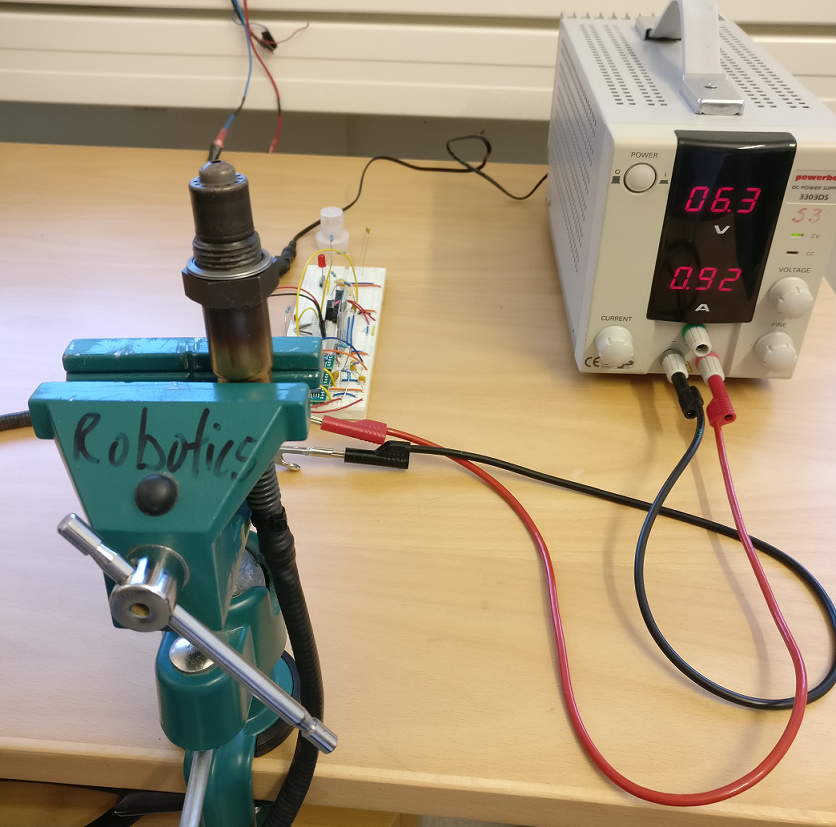
\includegraphics[width=.8\textwidth]{Chapter3/Figures/lambda_bench.png}
    \caption{Lambda sensor mounted to a vise.}
    \label{fig:lambda_bench}
\end{figure}


\subsection{Setup for programming}

Initially a PIC18F26K20 was intended to be used as \ac{mcu}. This is the same \ac{mcu} used in the radio system developed by Electrotech. However, with the need of two different I2C connections and to avoid bit banging it was later changed to a PIC18F26K22~\cite{PIC18}. Bit banging is a software technique for serial communication, when no dedicated hardware is available. This PIC is similar to the first one, but one difference is that it has two \ac{i2c} protocols. The processor was first ordered with \ac{dil}, this to get more familiar with them and it made it possible to connect them on a breadboard, which worked as a development board in this case. The PIC requires a separate device for programming the device. An ICD 3 (In-Circuit Debugger) is the link between the PIC and a Windows platform, it can be used for both programming and debug most of the PICs and was suitable for this project~\cite{ICD3}.





\section{OrCAD simulations}

\begin{figure}
    \centering
    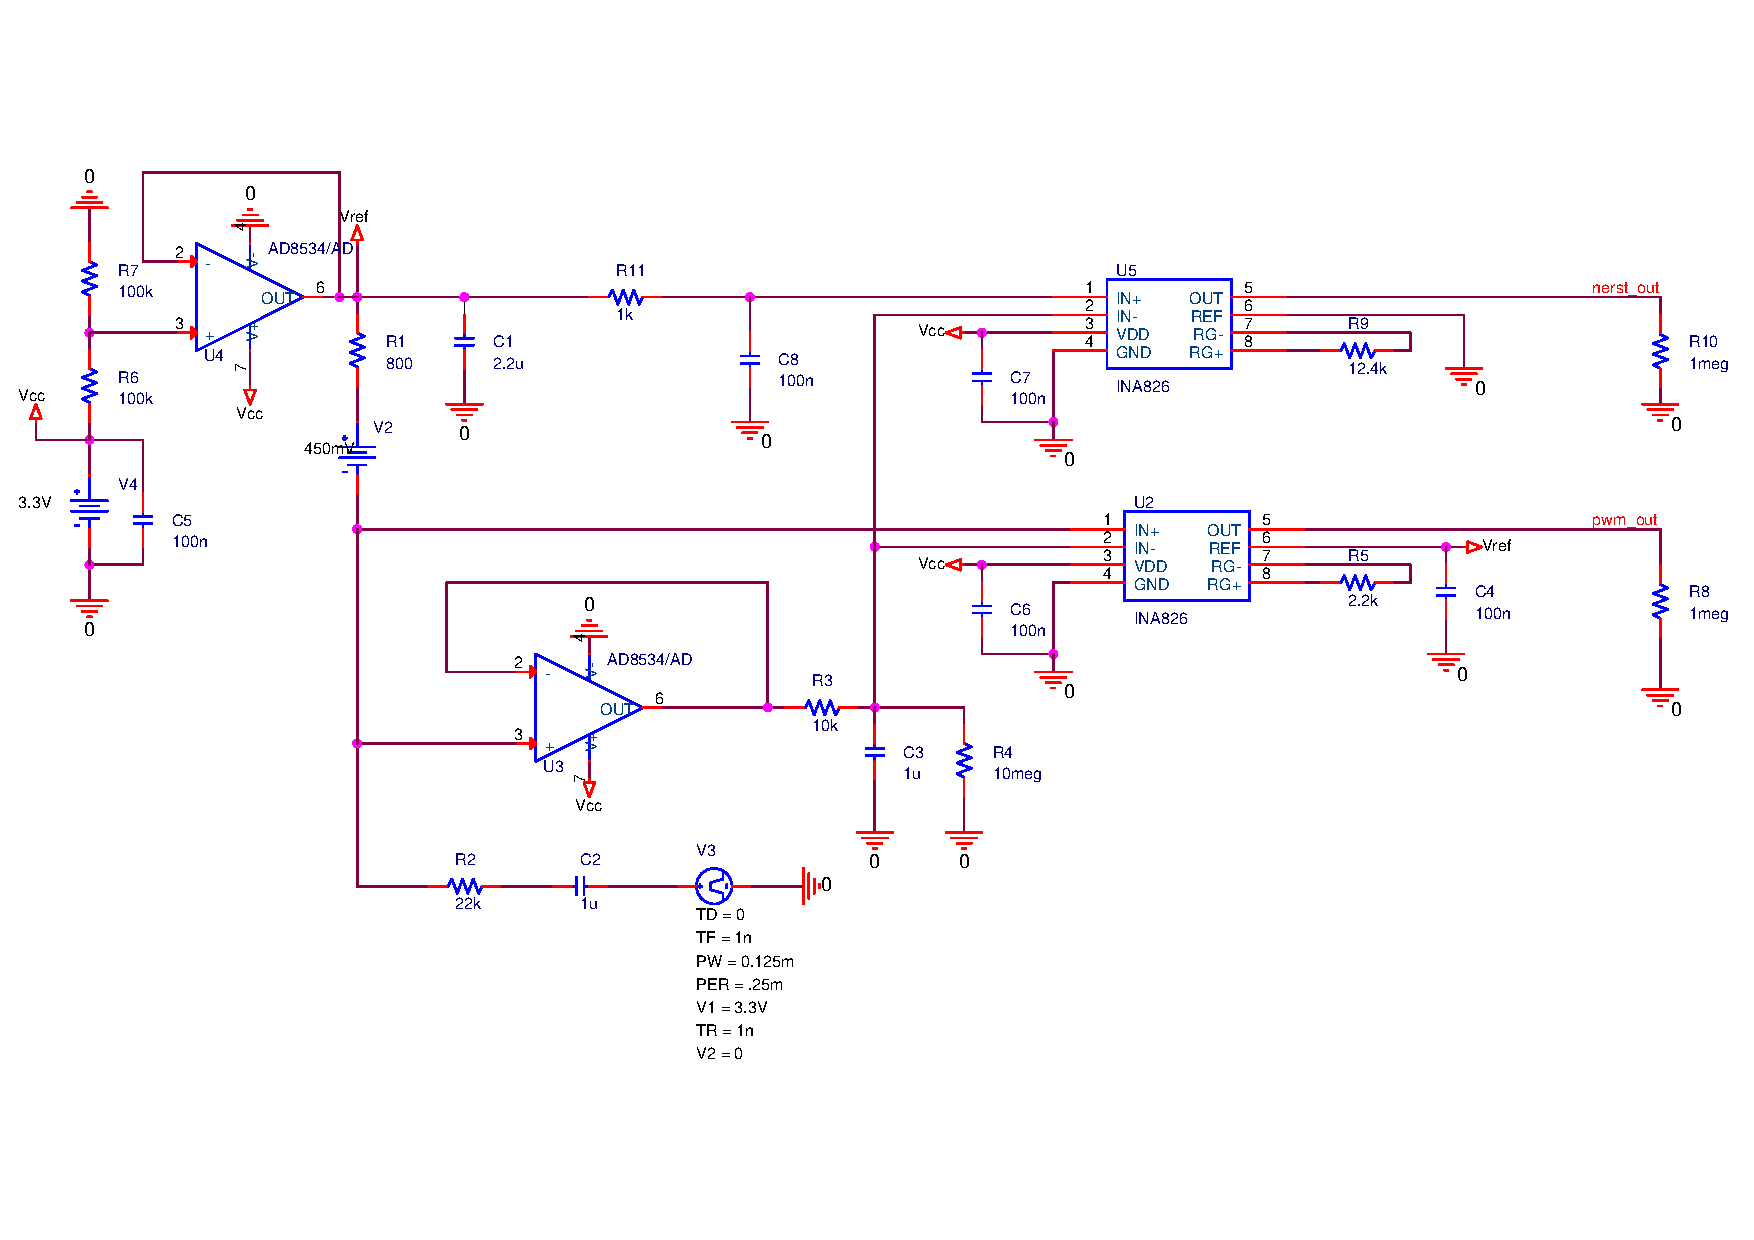
\includegraphics[width = \textwidth]{Figures/SCHEMATIC1_orcad.pdf}
    \caption{OrCAD schematic for nernst cell and instrumentation amplifiers used for measurement.}
    \label{fig:schematic1_orcad}
\end{figure}


By assuming that the sensor was in its operation point during the simulations in OrCAD, the pump-current could be neglected. This simplifies the simulation model and the nernst cell then acted like a voltage source stable at 450 mV. After these simplifications, the schematic looked like figure \ref{fig:schematic1_orcad}.


Over the nernst cell there are two measurements which are of interest. Firstly, one wants to measure the voltage drop over the cell, which is stable at 450 mV if the current regulator behaves as expected. An instrumentation amplifier takes the voltage difference over the nernst cell and amplifies it about 5 times to get a higher resolution on the 10 bit \ac{adc} pins available on the PIC.

The second measurement of interest is the resistance over the nernst cell. Because the cell is held at a constant \ac{dc} level of 450 mV, this measurement is instead done by doing a voltage division of an \ac{ac} signal. This \ac{ac} signal is generated by a \ac{pwm} signal from the PIC, and by supply it to a known resistance and the nernst cell in series, the resistance is calculated by measuring the voltage level between the known resistance and the nernst cell.

The first plan was to run the sensor on 3.3 V because of simplifications in the future if the sensor electronics are integrated in same electronics as Electrotech's radio transceiver. However, because of some battery limitations it was later changed to run on 5 V although all simulations are for 3.3 V.

%Because the temperature is measured with a PWM signal and the temperature in the oven will be kind of stable for long intervals, the temperature will only have to be measured now and then with a high sampling period. With this thought it was first supposed to only send a PWM signal in bursts when the temperature were going to be measured. However this may cause some problem and inaccurate readings, because the PWM signal goes from 0-3.3V it will generate a DC level on about 1.65V and when the DC level are implemented in the circuit it will take some time for the circuit to become stable and no readings should be made during this stabilising process and this may cause problem because the nernst cell will have to be continuously read to be able to control the current so the nernst cell will have a stable voltage.

\subsection{PWM signal}

It is expected to have a stable temperature of the sensor in the oven. Only the oven is heating up the sensor, so the temperature changes are most likely small over time, compared to if the heating element heats the sensor. Thus the first thought was to only measure the temperature in long intervals, by sending a \ac{pwm} signal in burst while measuring the temperature. Then, the amplitude of the \ac{pwm} signal represents the nernst cell resistance, which represents the temperature of the nernst cell.

However this may cause some problems and inaccurate readings, because the PWM signal goes from 0-5 V. It generate a DC level of about 2.5 V and when the DC level is supplied to the circuit, it takes some time for the circuit to become stable and  no readings during this stabilising process are preferable. This may cause problems because the nernst cell is continuously read, so for the current regulator for the pump current which holds the nernst cell voltage stable, there is a time frame with unexpected behavior.


One alternative is to send the \ac{pwm} signal during all time the system is active and taking measurements. But the \ac{pwm} signal is causing a noisier signal over the nernst cell and that can disturb the nernst voltage measurements.


Because of this issues both methods were tested to be sure which would give the best accuracy of the sensor readings.


\section{Temperature measurement on prototype board}

After the OrCAD simulations \ac{ic} adapters to build the circuit used for the temperature measurement over the nernst cell on a breadboard became useful. Before connecting the real lambda sensor to the breadboard a resistor of 220 $\Omega$ simulated the nernst cell resistance to see if the \ac{pwm} signal was correctly divided and amplified in the circuit. At first, the output signal which was connected to an \ac{adc} pin was just noisy and there was no characteristic of a \ac{pwm} signal. The decoupling capacitor on the virtual ground was then replaced by a bigger capacitor because this signal was also a bit noisy. After the change it was easy to see the measured \ac{pwm} signal. However it was still a bit noisy and one has to consider that when building the final board if it should be increased even more or if there is other reasons for the noise, or if it decrease only by building it on a PCB, which makes everything tighter.

The test resistance was then replaced with the lambda sensor and the sensor was heated with a power supply, where the voltage was controlled to not exceed the recommended heat up restrictions stated in the datasheet for the lambda sensor. When the heating element was supplied with 6 V, the measurement still showed the maximum \ac{pwm} output signal, going up to 6.4 V it decreased so the amplitude stated an resistance a bit below 1k$\Omega$, which represents an internal temperature of about 650 $\circ$C. The output signal is still a bit noisy, so to get a more accurate value, some more noise has to disappear.


\section{Breadboard run with major parts of the sensor circuit}

After being able to measure the temperature and communicating with the \ac{dac} through \ac{i2c} some tests were done on the sensor with most of the components mounted on a breadboard. The \ac{dac} could be controlled with the phone through a bluetooth terminal and the HC-06 module to the PIC18's eusart pins. It was controlled by either writing a "+" or "-" were the signs represented small steps up/down for the voltage. After some debugging and errors it turned out that the voltage drop over the nernst cell went the opposite way than expected. This caused the value for the voltage drop over the nernst cell to remain at 0 V when it in fact was increased. The reason was found to be that the differential amplifier stage was implemented with reversed connections on IN+ and IN-, which was later corrected.

\begin{figure}
    \centering
    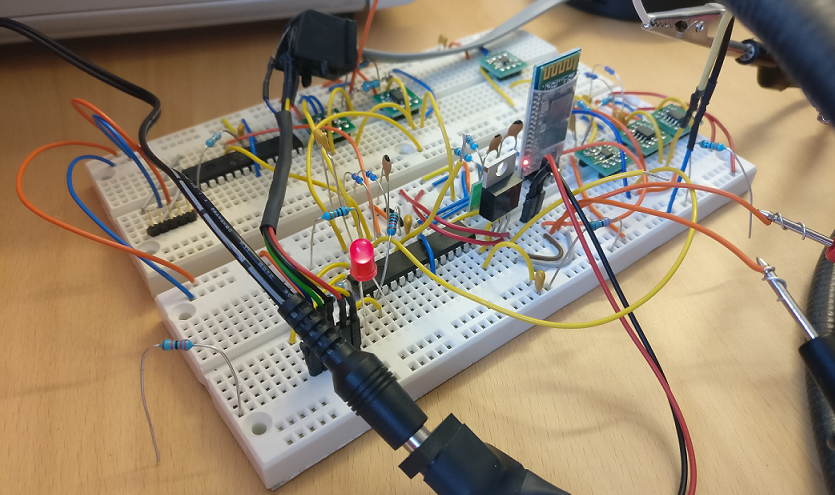
\includegraphics[width=.6\textwidth]{Figures/breadboard.png}
    \caption{Most of the functionality connected and tested on a breadboard.}
    \label{fig:breadboard}
\end{figure}


\section{Schematic description}

\subsection{Power supply}

There are two transistors used for power switching as shown in figure~\ref{fig:supply_schematic}. One switch is controlled by the PIC processor and the other switch can be controlled by an external device.

This second switch was meant to power down all supply and therefore end up with almost no power consumption when the power was cut off. It was meant to be connected to the radio module, which could then decide when to power on or off the sensor system. This second switch was bypassed however, so the PIC always had access to power supply. Sleep mode was instead invoked when no I2C command was received from the radio module.

The PIC then controlled the first switch which it turned off before entering sleep mode and switched on when it wake up and started to take measurements.


\begin{figure}
    \centering
    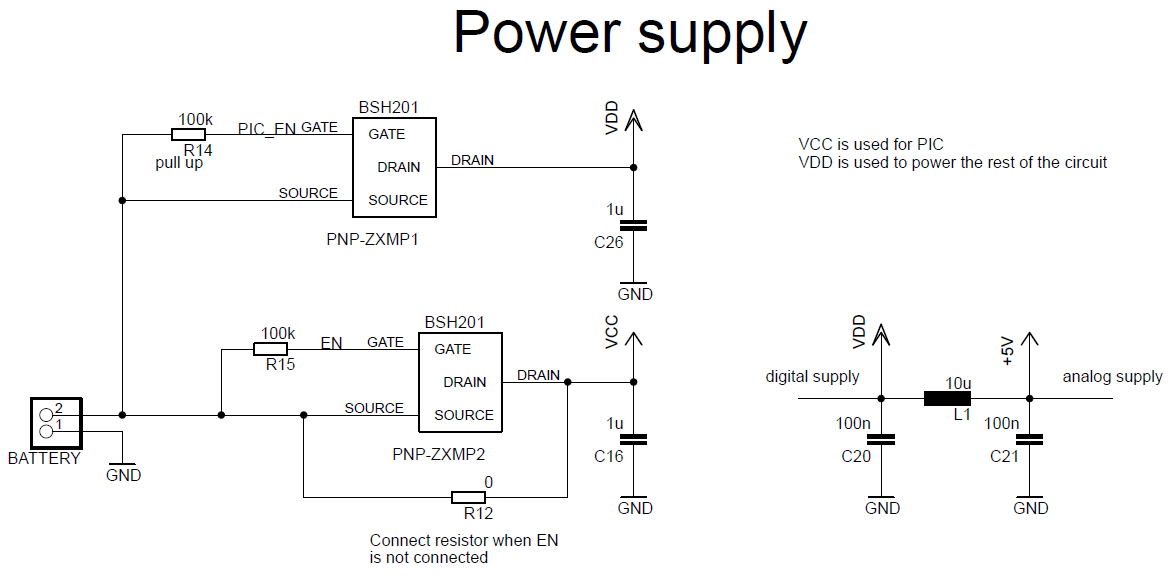
\includegraphics[width = \textwidth]{Chapter3/Figures/supply_schematic.png}
    \caption{Power circuit for PCB.}
    \label{fig:supply_schematic}
\end{figure}


\subsection{DAC for current regulation}

The DAC controls the current supplied to the lambda sensor and its schematic can be seen in figure~\ref{fig:DAC_schematic}. It is provided with a LC-filter on the output, where a ferrite inductance is placed over the gap between the digital and analog ground. The device is a 12-bit AD5622~\cite{AD5622} DAC supporting I2C communication, where the 12-bit value is linearly distributed between ground and supply. The capacitors added to the I2C lines are optional and was added because they stabilised the communication when the system was connected to a breadboard. It was not found necessary to use them on the final \ac{pcb} design.


\begin{figure}
    \centering
    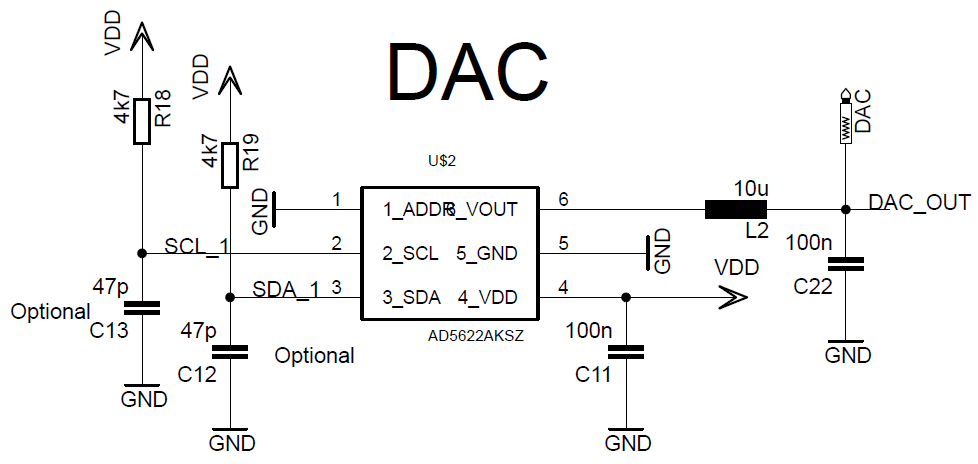
\includegraphics[width=.9\textwidth]{Chapter3/Figures/DAC_schematic.png}
    \caption{Schematic for the DAC controlling the current to the lambda sensor.}
    \label{fig:DAC_schematic}
\end{figure}


\subsection{Operational amplifiers used as impedance buffers}

In total three operational amplifiers were used, and the schematics for them is seen in figure~\ref{fig:OPamp_schematic}. All three were connected to have unity gain and used as an impedance buffer. It is almost the same operational amplifiers, with the difference that AD8539 comes with two op-amps in one package.


When setting the virtual ground, two resistors is used as a voltage divider. Then this node is connected to a high impedance input pin on an op-amp which acts as an impedance buffer.


The pin named nernst cell (RE+)~\cite{LSU49} will hold both a \ac{dc} and \ac{ac} signal. To get a clean \ac{dc} signal, the \ac{ac} signal is low-pass filtered by an RC-filter. Before the signal enters the RC-filter, it goes through an op amp used as an impedance buffer. So the RC-filter does not have any influence on the original signal.


\begin{figure}
    \centering
    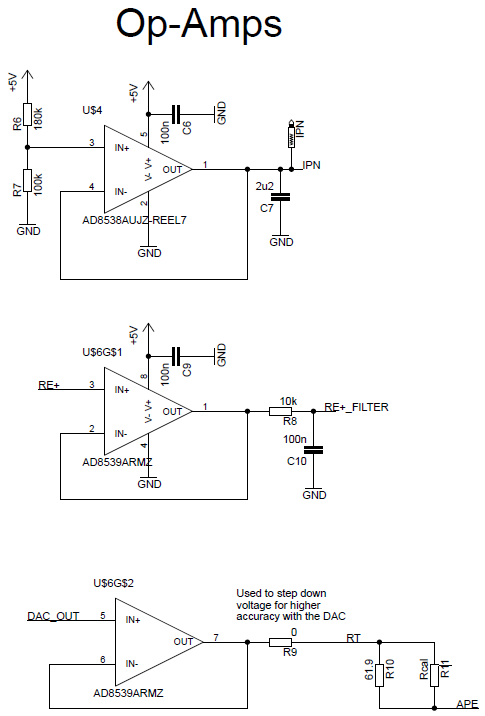
\includegraphics[width=.7\textwidth]{Chapter3/Figures/OPamp_schematic.png}
    \caption{Schematic for the three OP-amps used as buffers.}
    \label{fig:OPamp_schematic}
\end{figure}


\subsection{Instrumentation amplifiers}

The instrumentation amplifiers hold a circuit of three operational amplifiers within the \ac{ic}, where they connect in such a way that it takes the difference between two input signals and amplify it with a gain depending on one resistance. The output signal will then be the amplified difference between the input signals added to the reference point which the user set to a level between ground and supply on the reference pin.

The differential signals compared with an instrumentation amplifier, in this case, are the nernst voltage compared to virtual ground and the pump current, which is done by measuring the voltage drop over a 61.9 $\Omega$ resistance. The third amplifier compares the PWM signal entering the nernst cell with a low-pass filtered signal of the PWM signal. This to be able only to amplify the amplitude of the PWM signal before measuring it using an ADC pin.

In figure \ref{fig:INA_schematic}, the resistance connected between RG1 and RG2 on each amplifier sets the gain~\cite{INA826}, where the gain can be calculated by,

\begin{equation}
    G = 1 + \bigg(\frac{49.4~k\Omega}{R_G}\bigg).
\end{equation}

The reference pins on the amplifiers are connected to different points, depending on which signals that are compared. The nernst voltage is always supposed to be positive, and if so then the reference pin is connected to ground because then the output signal is always above the reference point.

The pump current can be negative, and therefore the reference pin is connected to virtual ground, which allows the instrumentation amplifier to amplify both a negative and positive difference on the input signals. The reference pin for the PWM amplitude amplifier also connects to virtual ground.


\begin{figure}
    \centering
    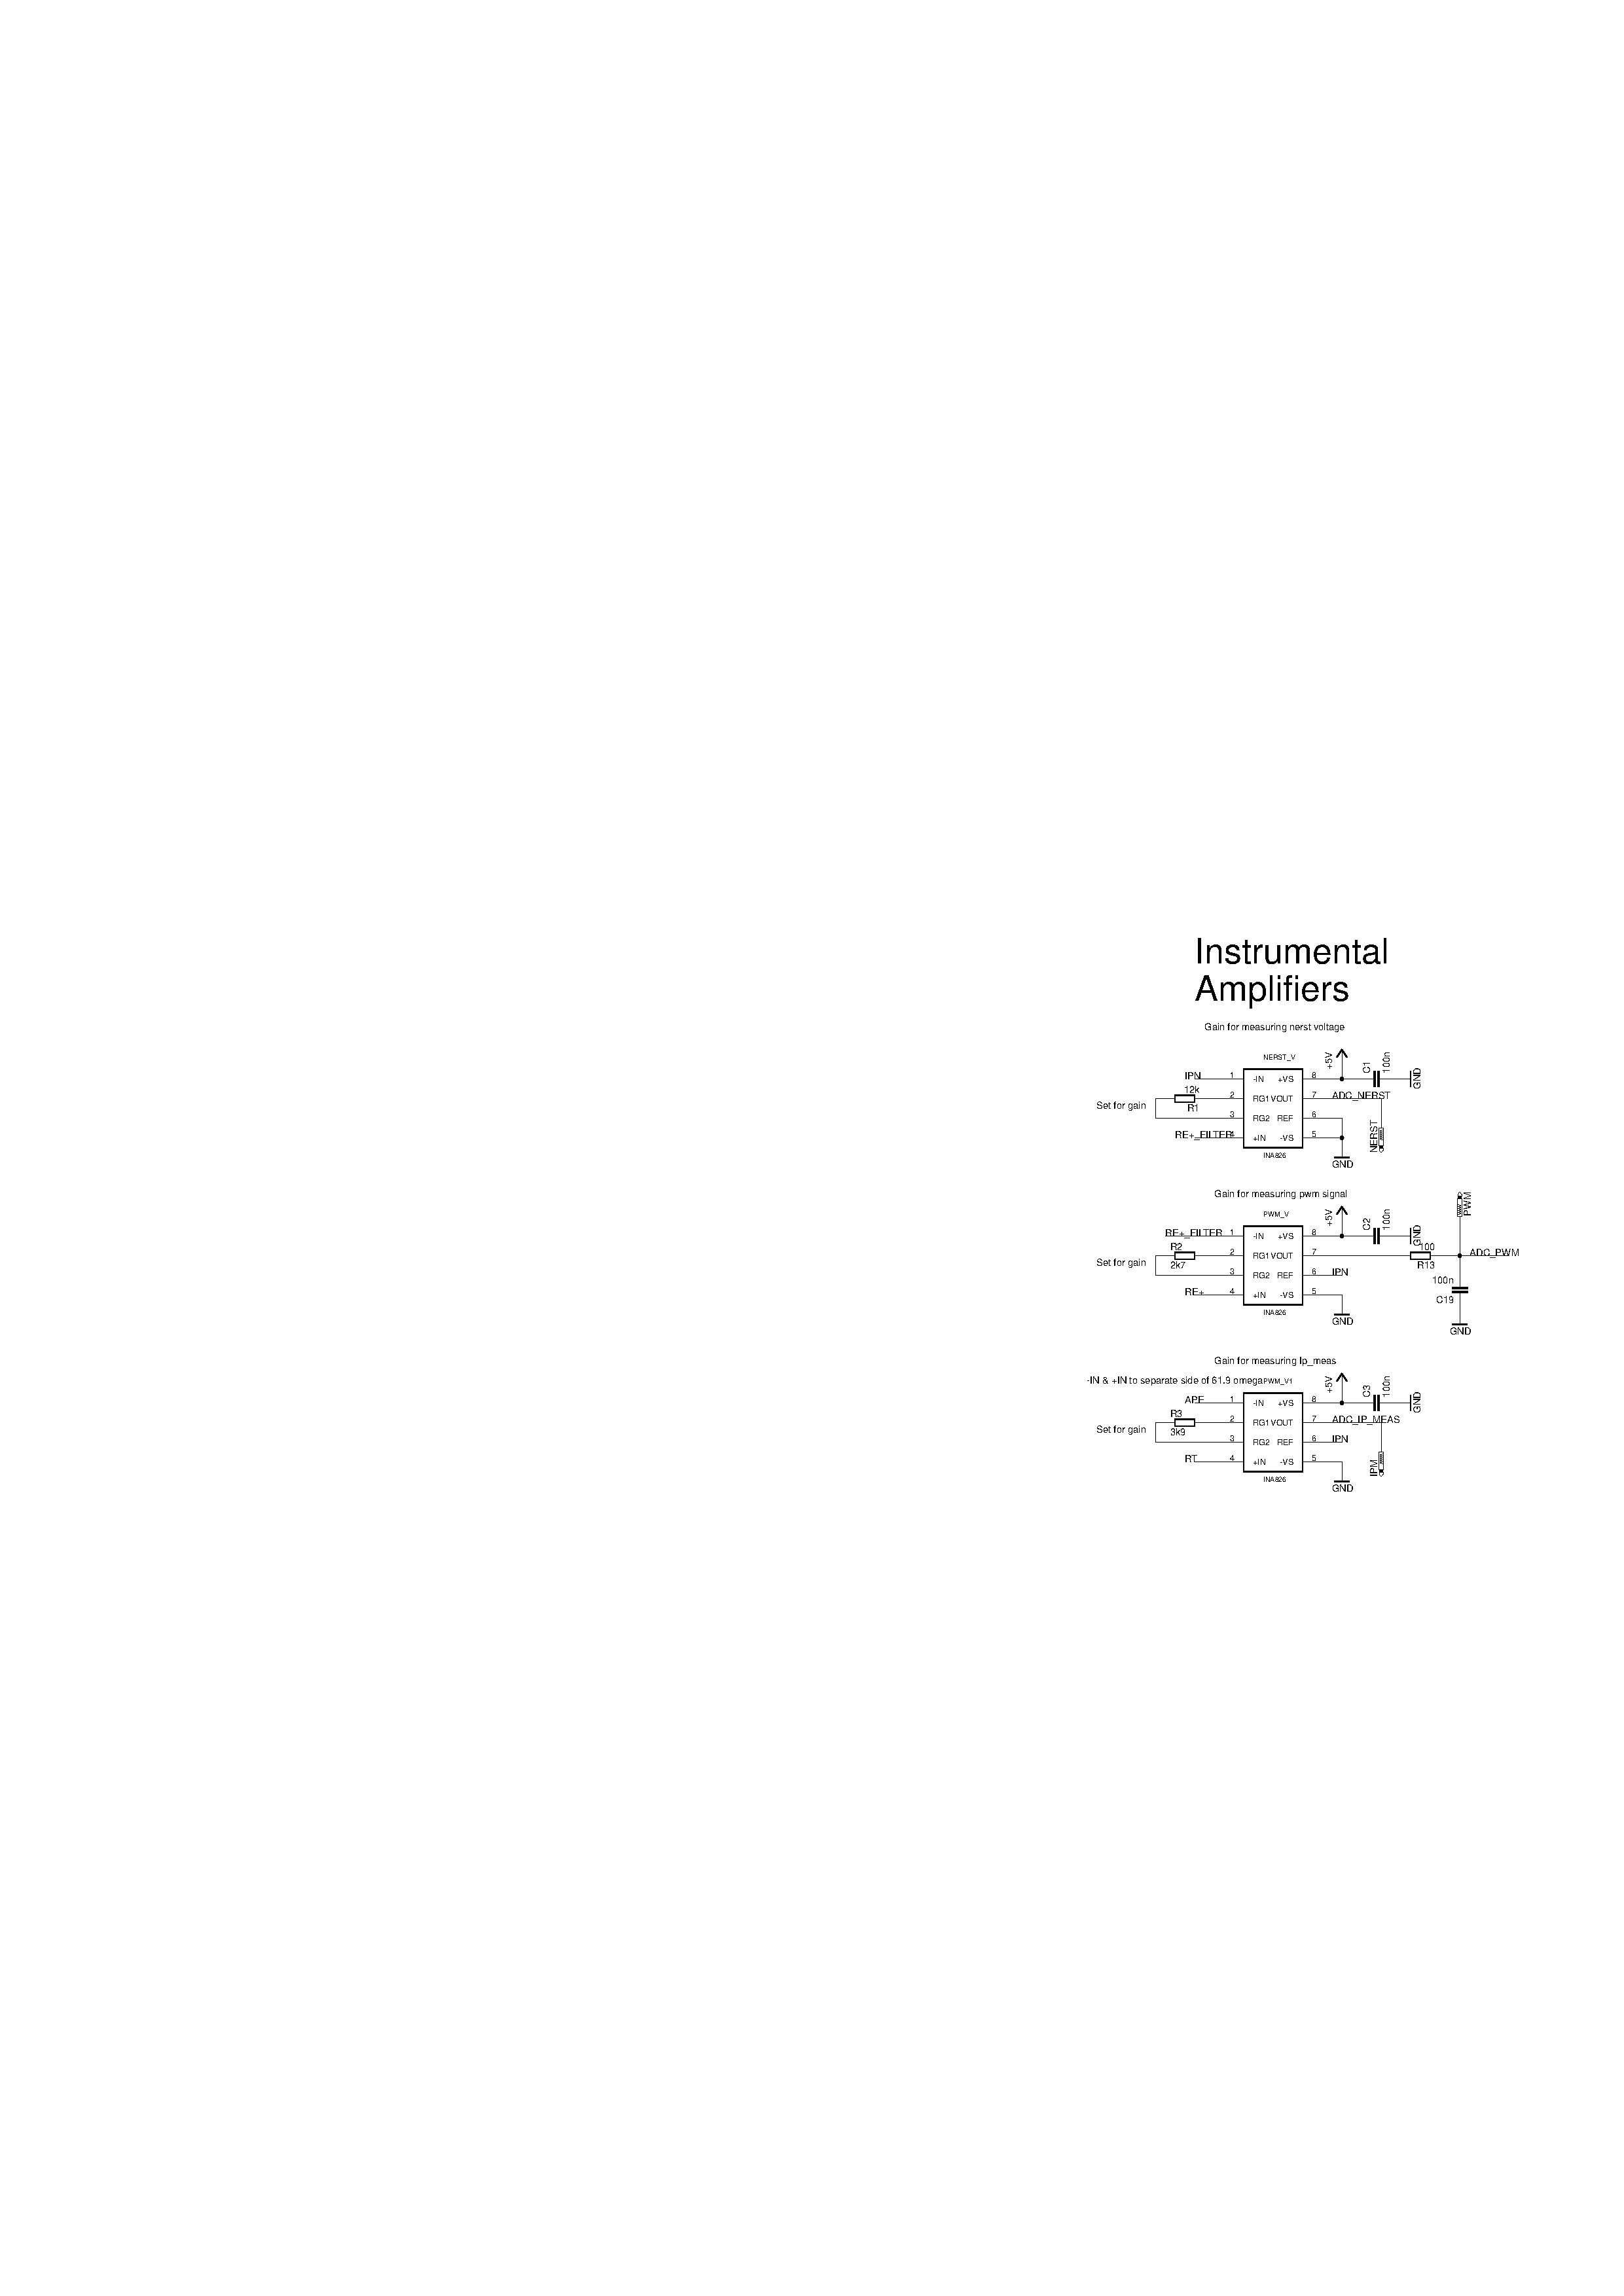
\includegraphics[width=.7\textwidth]{Chapter3/Figures/instrumental_schematic.pdf}
    \caption{Instrumentation amplifiers used for nernst voltage, pump current and temperature measurements.}
    \label{fig:INA_schematic}
\end{figure}


\begin{figure}
    \centering
    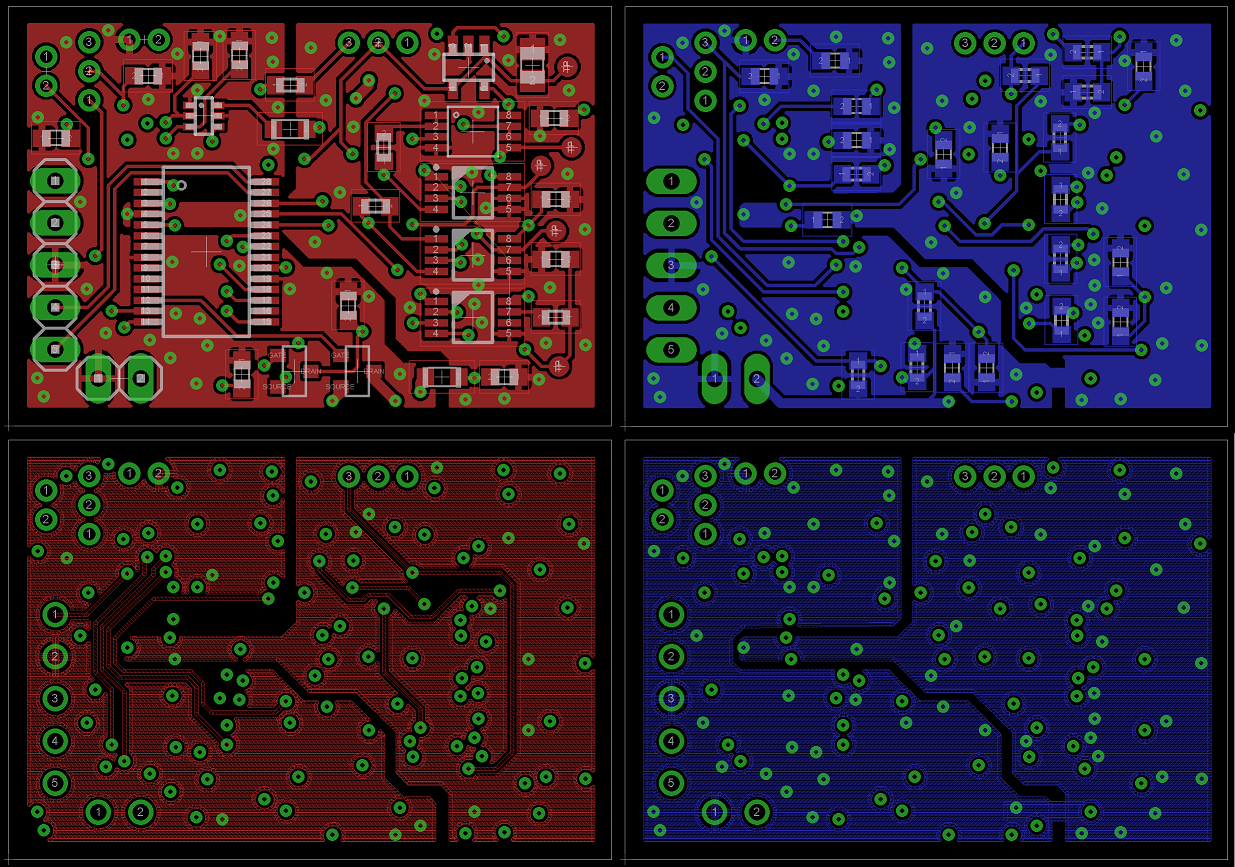
\includegraphics[width = \textwidth]{Figures/PCB4layer.png}
    \caption{All four layers of the PCB in Eagle. Red represents the two top layers and blue is the two bottom layers.}
    \label{fig:PCB4layer}
\end{figure}


\section{PCB design}

After simulating the circuit and running it on a breadboard, it was implemented as a schematic in Eagle~\cite{EAGLE}. The circuit already had some minor patches on the breadboard, which was taken care of on the schematic design in Eagle. The analog part of this circuit is the major part and also the most critical part to be able to get high accuracy on the measurement. A full schematic for the final \ac{pcb} design is found in appendix~\ref{appB}.

\subsection{Separating analog and digital signals}

The sensor system consists of mostly analog circuits. Here it is important that the analog signals don't get disturbed by the digital signals, to be able to have smooth and clean analog signals sent to the PIC. By splitting the ground plane into two parts and connect them at one node isolate the analog part. This method is called star-ground where several ground planes are connected just in one node. The analog part of the ground plane covers all analog circuits and the pins on the PIC where the analog signals are being handled.

This separation is done by doing a cut in the copper plane where all digital signals placed on one side of the cut and the analog signals placed on the analog part of the ground. However, one small path between the ground planes allows the analog and digital ground to be still connected to each other, see the dark blue picture in figure~\ref{fig:PCB4layer}. All pins used as analog pins on the PIC are selected, so they are close to each other, this because the PIC covers both the analog and the digital ground. So by having the analog pins close to each other, it simplifies the splitting of the ground plane.


There is also important to have a clean supply voltage, in particular for the analog circuit. To achieve clean and accurate analog signals is as little noise as possible on the analog supply wanted. The voltage from the battery is split in two. One supply goes directly to the digital voltage supply, and the other supply is connected through an LC-filter to prevent noise raised in the digital part to reach the analog part.

Also, all signals going from analog to digital part have a series resistance to prevent noise, this resistor is placed over the gap between the analog and digital ground.

\subsection{Dimensions}

Because there are some space limitations in the oven, it is beneficial to have a small \ac{pcb}. Therefore a \ac{pcb} with four layers is designed, because it makes it easier to place components on both sides and still have a good ground plane. On the two layers in the middle, there is one ground layer and one supply layer. In figure~\ref{fig:PCB4layer} the dark blue layer is the ground layer, and the dark red layer is the supply layer. The ground layer is free from traces. Keeping the ground layer free from traces allow the signals have the shortest possible circuit. The signals are then less likely to pick up noise. The outer dimension of the \ac{pcb} is 26x37 mm.

\subsection{Connector}

The following connections are available on the PCB,

\begin{itemize}
    \item Power
    \item Programming
    \item Lambda sensor (LSU 4.9)
    \item \ac{i2c} communication
    \item \ac{usart} communication
\end{itemize}

For the power and programming connectors, which is visible in the top corner in figure \ref{fig:monterad_PCB}, it use standard pin-header connectors with 2.54 mm pitch. This type of connection makes it easier to connect, disconnect and program the device. The device is under a development process, and that's why this simplicity is especially wanted. So if another \ac{pcb} would be designed as a finished product, these connectors would most likely be smaller.


The connectors for the lambda sensor, \ac{i2c} communication and \ac{usart} communication have all the same size on the connectors. This connection was not a good idea for the lambda sensor, since its wires are thicker than the connector holes and thus makes it a bad design. For the \ac{i2c} communication and \ac{usart} communications it was suitable. It could however be designed with a bit wider solder pad to simplify the soldering process.


\subsection{Component size}

Most of the passive components are 0603 components. 0603 tells the components dimensions in mills. 0603 components are small enough not to take too much space on the \ac{pcb}, but big enough to be soldered by hand with not too much of a hazard.

Most of the ICs used were available in both \ac{soic} and \ac{sop}, the \ac{sop} was selected to keep the size down. It should be possible to find a suitable transistor with a smaller package however.


\begin{figure}
    \centering
    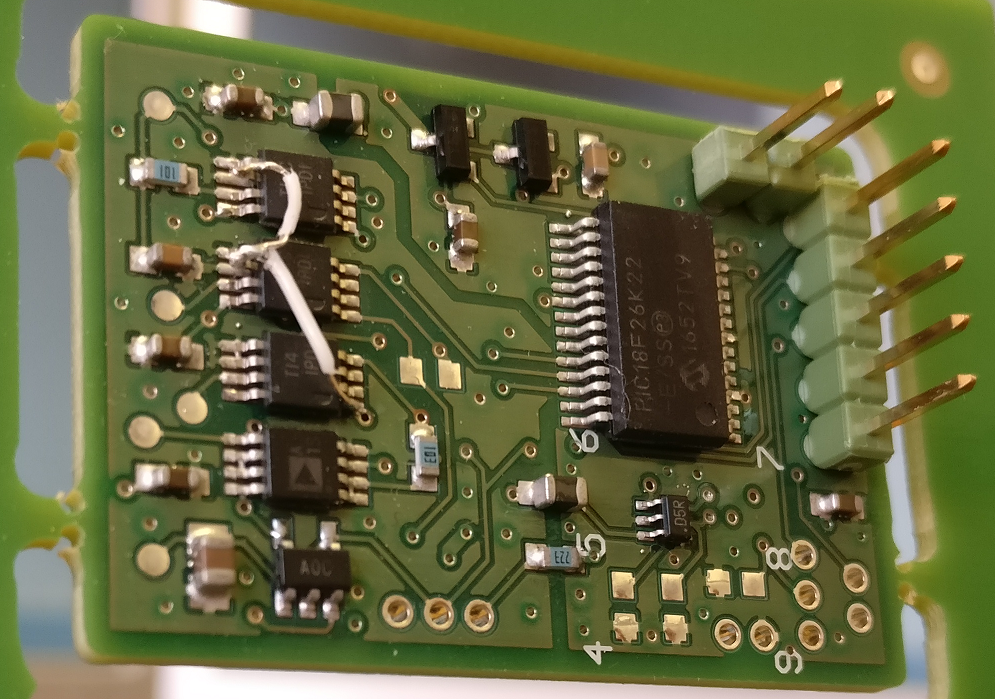
\includegraphics[width=.6\textwidth]{Figures/PCB_monterad.png}
    \caption{Mounted PCB.}
    \label{fig:monterad_PCB}
\end{figure}


\section{Operating voltage}

The operating voltage for the sensor was first decided to be 3.3 V. The system was then also designed for this voltage, but it didn't manage to run on a lower volt than 3.3 V in an oxygen rich environment. But Electrotech had some concerns that the used batteries which, could drop down below this limit. Because of this reason, two batteries were put in series and connected to a 5 V voltage regulator.

This change seemed not to be any problem because all electronics used for the sensor system were designed to handle up to 5 V. The system also uses the \ac{fvr} built into the PIC, to compensate for an eventual difference in supply voltage. However, the gain from the pumping current measurement and nernst voltage measurement was constant. With this follows that the voltages which are to be measured, don't follow the increment of the supply voltage from 3.3 V to 5 V. This gives a lower accuracy on these measurements if the gain is untouched and they are limited by the 10-bit \ac{adc}, which follows the supply voltage. 


\section{Communication between Radio system and Sensor system}

Electrotech has been adding space for four wires to connect to their system for the \ac{i2c} communication. Two wires used for the actual communication, one wire to have a common ground and the last wire for level conversion on the data and clock lines. However, since the system seemed to most likely run on 3.6 V unregulated, there would not be any need for a level conversion, because both systems would run on same supply level in this case and it would give us the opportunity to run on the same battery. But the supply was later changed to 5 V, and the level conversion was then needed.

\subsection{Communication protocol}

Electrotech gave us some opportunity to decide how we want the communication to be in some sense. The sensor system has to wake up from sleep or idle mode through an \ac{i2c} command. Then the radio system is pulling for data where we set up how the pulling should be implemented and then set up how we want to send the data. Then the data is then sent to their radio antenna.

The communication starts when Electrotech sends a start command (0x01). This command wakes up the sensor system which then responds with (0xff), which represent that no data are available yet. The sensor system stays awake and measures as long as Electrotech repeatedly sends request one time per second. When the sensor system has stabilized, it responds with 48 bits of data. 16-bits each for the oxygen concentration, sensor temperature and the nernst voltage.



%\section{Trip to Kalix 20170315}
\subsection{Test run in Kalix}

When both parts have been working on the communication on their own, it was time to verify that it worked as expected. It was tested in Kalix, and it didn't work from the start. By using an oscilloscope with built in \ac{i2c} decoder, able to display what the communication looked like on the oscilloscope was a useful debugging tool.

At the end of the day, the I2C communication worked in some sense. It looked correct on the oscilloscope, but some error in the software which not acted as expected. By doing an exchange of electronics, so both parts had access to all electronics used in the experiments, made it possible to work further from a distance. Hex-files of software could then be sent from one part to the other, who then reprogrammed their device.



%The main goal with this trip was to check if the communication between the sensor system and Electrotech's radio unit worked as expected. As mentioned before the communication protocol used was I2C. There were some struggle before it worked as expected with some minor bugs from both part. However, the one who was responsible for the communication from their part, had an oscilloscope on his office, which were able to read I2C protocol and it was a great source for the debugging process. At the end of the day we manage to setup the communication so it looked good on the oscilloscope, but Electrotech didn't manage to read the data and send it further by radio. This was most likely some bug from their part and they are going to send a software update when it is fixed. Because we did some exchange of hardware there will be easy to just send some software update to test when it is fixed.

\section{Tests performed in oven}

There have been three tests in an oven in total. The first test, which is also the biggest test, was in an oven where all the electronics were inside the oven during the test. This test lasted for about 2 hours, and all the electronics were surrounded by water for cooling properties, while the sensor was pointing out to the oven. 

The other two tests have been in a small oven. Here, only the sensor functionality was tested. In other words, the electronics were outside the oven and only the sensor was exposed to the oven. These tests were done to see how the sensor behaved in this kind of environment and to verify that the electronics were functioning.




\section{Building process in Kalix}

\subsection{Waterproofing of electroncis}

%After some concern however the sensor oxygen electronics will be able to run on 3.6V, the voltage level was increased to 5V. Because all electronics were design to handle some level shift without giving wrong measurement data, this wasn't a problem and all components were rated for 5.5V or more. The critical part by doing this was the level-shift on the I2C communication and this was implemented by Electrotech.

Water surrounded the electronics during the tests, which was used for cooling. Then the electronics were covered with some waterproof epoxy to keep all water away from the electronics, so the water only fulfills its cooling effects.

After testing all functionality and power consumption, the electronics were soldered together and tested before placing it in plastic boxes. The communication didn't work at first, but it turned out that data and clock lines were switched on the I2C communication. Figure \ref{fig:electronics_box} shows how all electronics placed in a plastic box, which later on was filled with some waterproof epoxy. The box was used to keep the epoxy in place before it hardened.



\begin{figure}
    \centering
    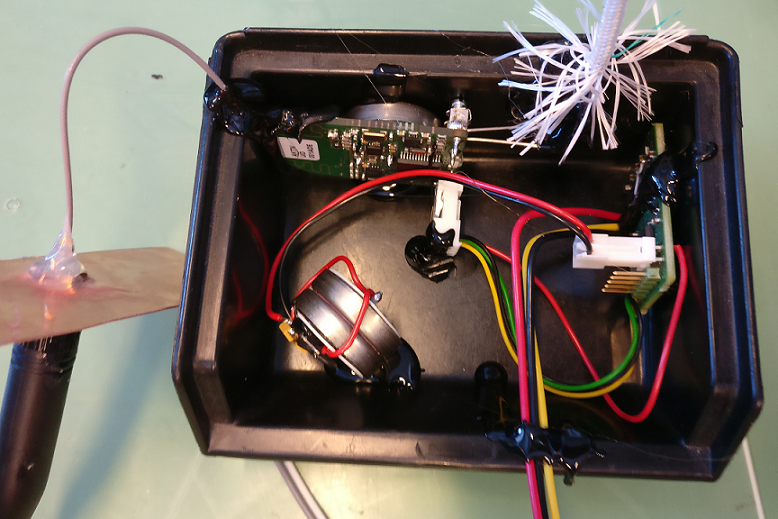
\includegraphics[width=.8\textwidth]{Chapter3/Figures/electronics_box.png}
    \caption{Electronics in plastic box before covered by epoxy.}
    \label{fig:electronics_box}
\end{figure}


\subsection{Mechanical design}


In figure \ref{fig:mechanical_construction} one can see how the system look before water surrounded it. In the figure, the system is upside down, where it during the test is flipped and surrounded by water. The white plate is isolation material and is the top of the system. It has one hole for the lambda sensor, one hole for thermocouple and some smaller holes where water vapor can escape.


All electronics and sensors were mounted to be stuck on the top plate, so all equipment is held in place even when the plate is flipped. It was then placed on top of the box in figure \ref{fig:water_box}, which contains some water foam. The water foam absorbs water and prevents water spill when the system is moving. The box in its turn was surrounded by isolation material, to delay the water being heated up. When the water reaches 100 $^\circ$C, it stays at this temperature until all water has boiled away. This temperature is also the reason all electronics are rated to last at least 125 $^\circ$C.


\begin{figure}
    \centering
    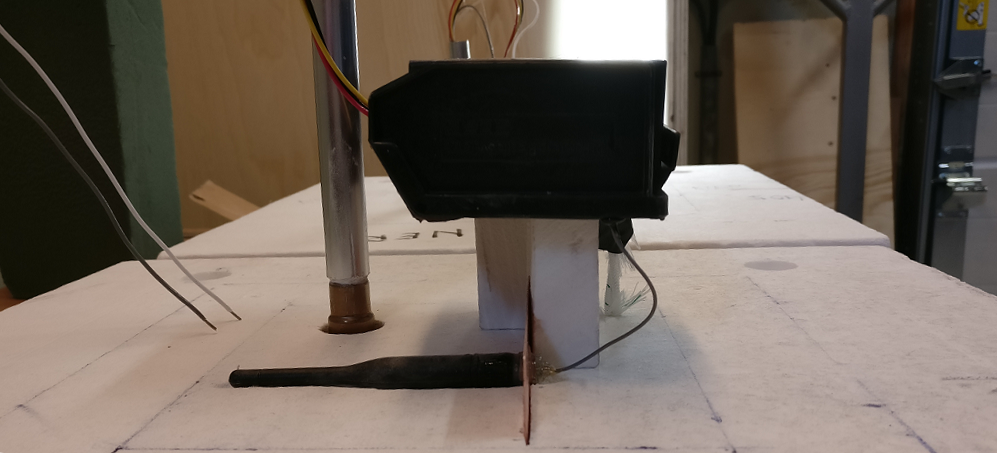
\includegraphics[width=.8\textwidth]{Chapter3/Figures/mechanical_construction.png}
    \caption{The mechanical design for the system.}
    \label{fig:mechanical_construction}
\end{figure}


\begin{figure}
    \centering
    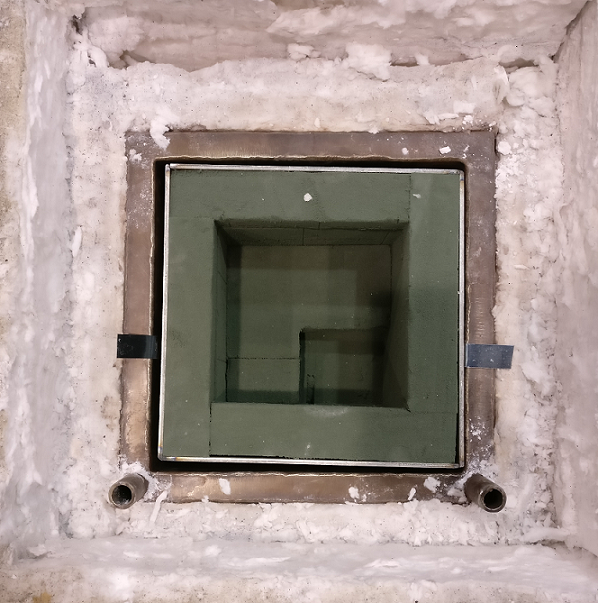
\includegraphics[width=.7\textwidth]{Chapter3/Figures/water_box.png}
    \caption{Metal box filled with flower foam and surrounded by high temperature isolation material.}
    \label{fig:water_box}
\end{figure}


\section{Controller for pumping current}

The pumping current has to be regulated so that the nernst voltage is stable at 450 mV. A controller is implemented for the current to hold this nernst voltage stable. On the first test at Mefos, a simple controller was used, which decreased or increased the current with fixed steps depending on whether the nernst voltage was higher or lower than 450 mV. This method worked fine in normal room conditions, where the oxygen level is stable and there is almost no disturbance. It didn't work well in the oven at Mefos where the conditions were a bit worse and there were faster changes in oxygen concentration.

For the second try a \ac{pid} controller was implemented. A \ac{pid} controller depends on three variables. The proportional error (P), the integrated error (I) and the derivative change of the error (D). When designing this controller, it was heavily weighted to depend much on the proportional error. At first, the I and D parts were set to be zero, and the P part was increased as high as it could before it started to oscillate. Then it was lowered a bit and the I part was increased a bit. The I part had some strict saturation limits to avoid overshoot and oscillation. It was mainly used to fine tune the current when the nernst voltage was close to 450 mV. Then the D part was increased until the controller started to oscillate, then lowered some. 


In the second small test at Mefos and the best test so far, a \ac{pi} controller was used instead. It is easier to tune than a \ac{pid} controller and it performed well enough for this application.




\section{O\texorpdfstring{$_2$} ~~calculations}


The oxygen concentration depends on the current drawn by the lambda sensor. When the nernst voltage is stable at 450 mV and the sensor has correct temperature, the relation between the current used by the sensor and oxygen concentration is described as figure \ref{fig:o2ipmeas}~\cite{LSU49}.


\begin{figure}
    \centering
    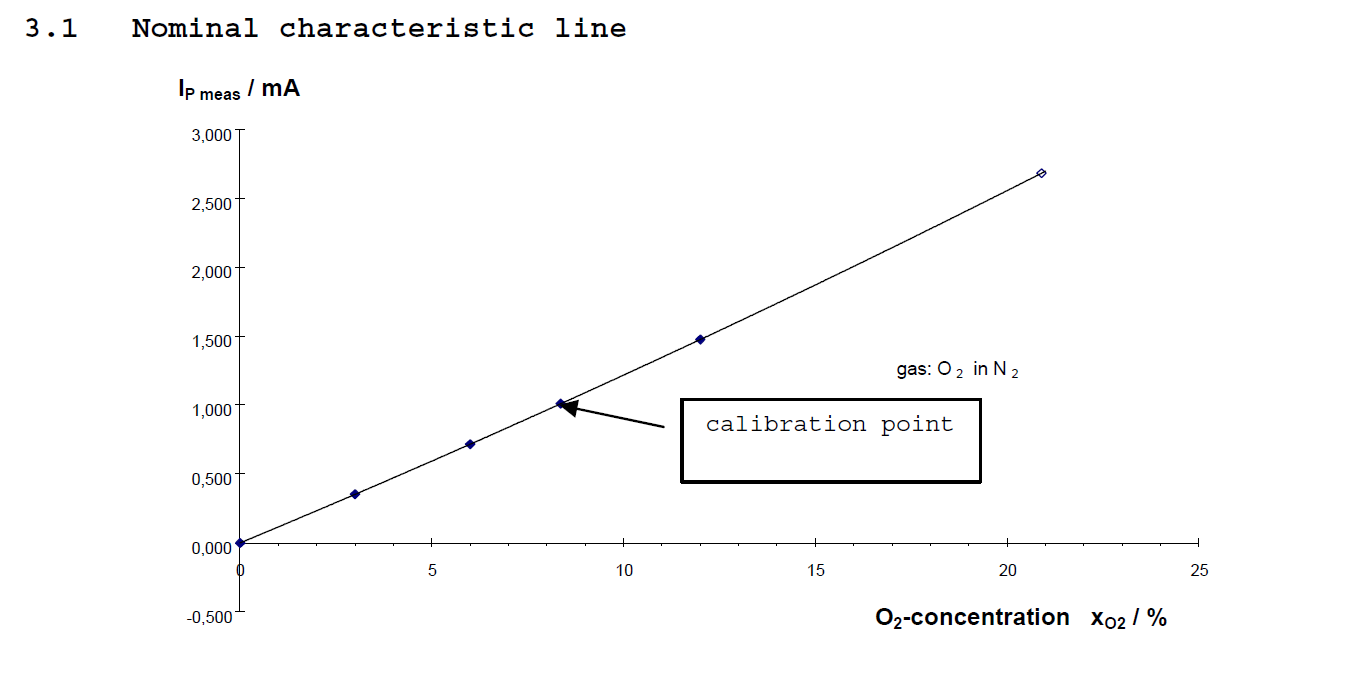
\includegraphics[width=\textwidth]{Chapter3/Figures/o2ipmeas.png}
    \caption{How the O$_2$ concentration depends on Ip$_{meas}$.\cite{LSU49}}
    \label{fig:o2ipmeas}
\end{figure}


Figure~\ref{fig:o2ipmeas} is provided from table~\ref{tab:o2ipmeas}, which is found in the datasheet for the lambda sensor~\cite{LSU49}. Ip$_{meas}$ is measured over a 61.9 $\Omega$ resistor, located in parallel with the trimming resistor calibrated for each lambda sensor in figure~\ref{fig:schematic_lsu49}.


\begin{table}
    \centering
    \caption{Relations between oxygen concentration and current used by lambda sensor.}
    \begin{tabular}{|l|r|r|r|r|r|r|} \hline
         O$_2$-conc. x$_{O2}$ [\%]    &  0    &  3.0 & 6.0    & 8.29  & 12.0  & 20.95  \\ \hline
         Ip${_meas}$ [mA]              &  0    & 0.33 & 0.67   & 0.94  & 1.38  & 2.54  \\ \hline
    \end{tabular}
    \label{tab:o2ipmeas}
\end{table}


\section{Software}

The software is designed for a PIC18F26K22~\cite{PIC18} and developed in MPLAB X IDE v3.51~\cite{MPLAB}.

\subsection{Overview}

Figure~\ref{fig:Software_map} gives an overview over the functionality of the software. At first, when the system starts, it initialises all the functions. It sets the pins to match its purpose, and initialise properties such as \ac{i2c}, \ac{adc} and \ac{pwm}.

Then while it waits for an \ac{i2c} interrupt from the radio unit, it constantly measures the nernst voltage to be able to control the pumping current for the sensor. If no \ac{i2c} interrupt happens within approximate 3 seconds, the system enters sleep mode. The system is brought back to an active mode when it receives an \ac{i2c} interrupt. When this happens, it sends its latest measured values from the nernst voltage, pumping current and \ac{pwm} amplitude through \ac{i2c} to the radio unit. The pumping current is used to calculate the oxygen concentration and \ac{pwm} amplitude for temperature calculations.

After the values have been sent, the system updates all values and then goes back to constantly measure the nernst voltage to regulate the pumping current for up to 3 seconds if no interrupt is received.

While the radio unit is active, it creates \ac{i2c} interrupts one time per second, and to ensure the sensor system is active during this time it waits 3 seconds before it enters sleep mode. When the sensor system enters sleep mode, it cut off the power to all components except the PIC. This is done by setting the gate high on a \ac{pmos}, which is used as a power switch.



\begin{figure}
    \centering
    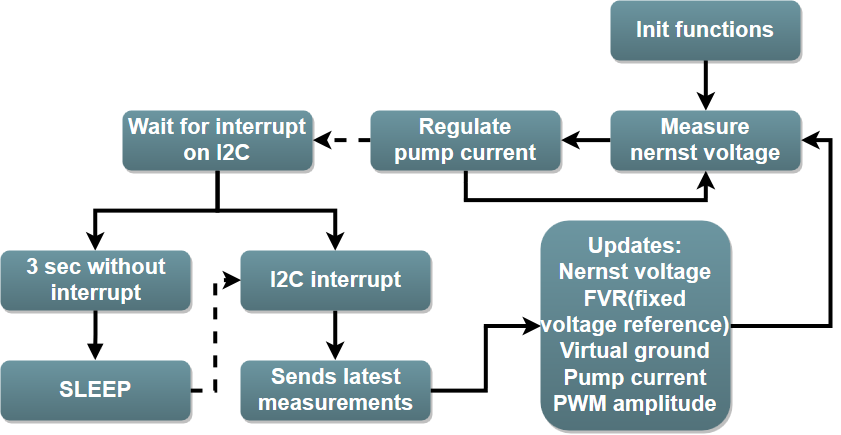
\includegraphics[width=\textwidth]{Chapter3/Figures/Software_map.png}
    \caption{Block schematic illustrating software functionality.}
    \label{fig:Software_map}
\end{figure}


\subsection{ADC measurements}

The \ac{adc} measurements which are done but not sent to the user, which also is shown in figure~\ref{fig:Software_map} is the \ac{fvr} and virtual ground. 

The virtual ground is measured to calculate the correct voltage difference entering the instrumentation amplifiers. This because the virtual ground is used on the reference pin on the instrumentation amplifiers. Then the output voltage is the voltage difference between the input signals added to the virtual ground. Then one has to subtract the virtual ground from the output measurement to be able to calculate the correct input difference.

The \ac{fvr} measurement is used to calculate the supply voltage for the sensor system. This voltage reference is set to be stable at 2.048 V, and by measuring the \ac{adc} value of this voltage, one can calculate which supply voltage is used. This is then used to compensate for differences caused by the supply voltage on the \ac{adc} measurements.



\subsection{Interrupt handler}

The interrupt handler has two different priorities. High and low priority.

An \ac{i2c} interrupt caused by the radio system generates a high priority interrupt and this communication is done within this high priority interrupt handler. Because this interrupt has the highest priority, all other interrupts happening during this time are put in a queue and is not handled before the high priority interrupt is done.


A low priority interrupt is caused by,

\begin{itemize}
    \item ADC conversion
    \item Timer4 interrupt
    \item Compare5 interrupt
\end{itemize}

The ADC interrupt is generated when a conversion is done and the ADC buffer holds a new 10-bit value. It then enters the low priority interrupt and clears the flag for ADC interrupt. The calculations for the ADC interrupt are then done in the main code.

When a Timer4 interrupt is generated it is done in the same way as the ADC interrupt, where it clear the flag and then returns to the main code, where calculations for the Timer4 interrupt are done. The Timer4 interrupt is used to start an ADC conversion on the nernst voltage.

The Compare5 interrupt is handled directly by the low priority interrupt handler. It is used to start an ADC conversion for the PWM amplitude, and the Compare5 register is comparing the clock value from Timer2 which is used for the PWM duty cycle and frequency. Then this Compare5 register guarantees that the ADC conversion for the PMW amplitude is done when the PWM signal is high and low to be able to calculate the amplitude of the signal.

\subsection{Measurement order}

\subsubsection{During the first test at Mefos}
When the sensor system is active and taking measurements, it will constantly be measuring the nernst voltage to be able to calibrate the Ip current which is used to decide what oxygen concentration it is in the environment.

When a request for data was received from the radio unit, the sensor system first sent it newest measurement values. Then it updated all values starting with the fixed voltage reference, followed by virtual ground, Ip current and temperature measurement. After this, it went back to calibrate the Ip current by constantly measure the nernst voltage. How often it measured the nernst voltage was decided by the Timer4 interrupt on the PIC. This interrupt was set to be generated 60 times per second.


\subsubsection{During the tests in the small oven at Mefos}
The measuring order was changed a bit in these tests, compared to the previous. One difference was that the temperature was only measured one fifth of the times compared to the other measurements. The generated PWM signal was only activated during this measurement. The reason for this was to decrease the potential of noise on the other measurement being caused by the PWM signal.

The other difference during these tests was the number of measurements. This time each measurement, except for the nernst voltage, was done 8 times between each I2C request. The mean value from these measurements was sent to the user. The nernst voltage was measured continuously during all time the system was active. When the nernst voltage was sent to the user, it was the mean value from 8 of the measurements between the I2C requests. At the first test, only one measurement was considered when it was sent to the user.



\section{Test and fault search on system}


When everything was built together and the system was tested in normal tempered air and heated up with a power supply, it didn't work. The nernst voltage was at its bottom and the \ac{dac} didn't increase the current. Some temperature cycles on the sensor were then made with a power supply. The temperature was changed in such a way, the sensor went from not operating temperature to operating temperature for some iteration and it started to work after a while then.


This caused some major concerns however the system would be able to run in the oven or not. 

By doing some fault search and attempts to recreate this error, it seemed at that moment like the sensor system had a lower chance of running correctly after it waked up from sleep mode. 

At the test day with this information, the sensor was heated up with a power supply and confirmed it operated correctly. Then it was left in its active mode during the rest of the time before it entered the oven and inside the oven as well.


The fault searching continued after the test and it turned out that the error was within the software for the current regulator. It caused an overflow on the 12-bit \ac{dac} value, where the software thought it was sending its maximum value, but this value was 0 V for the \ac{dac}.


%When the two setups of sensors was first run in Kalix, it didn't work from start. But after some mixture with the temperature, both system started to give good oxygen values. In these cases it seemed like they started to give correct values on a sharp temperature rise event on the sensor.

%These tests in Kalix was on a Friday and the setups were tested once more in Lule\r{a} on Monday and for the first system it didn't worked at first. But after some temperature cycles it started to work. But this time it started to give good values when the temperature already was high and not during a sharp temperature change and that was for the tag 1ADF

%On the next sensor setup it will be tested if the system will start working if it is left with a high temperature for a while, without changing the temperature or anything when it already is high. This system have the tag 1ADE

%The other system start working immediately on the Monday trial and it have the tag 1ADE 


%There were some thoughts that some contaminants might have damage the sensors, during the mechanical built up phase. The sensors were mounted to the isolation material with a epoxy and soft isolation material. Therefore we used a test sensor that was mounted to a test piece with the same method and afterwards the sensor still worked, which lowered the change for the epoxy to damage the sensor.

%After some readings that silicon is harmful for the sensors, a similar test was performed where the sensor had to "breathe" silicon for 15-20 minutes before it were tested. Silicon were used in our case to mount a aluminium pipe to the sensor, which would increase the cooling performance for the sensor. The sensor stilled worked after this test also though. 

%The fault searching resumed after the test with the debugger connected to the system. The error were reproduced after some heating cycles. When it was reproduced, the bias points were measured with a oscilloscope and it turned out that the fault was in the software controller for the pumping current. It caused an overflow to happen, which caused the DAC to send out 0 V instead of 5 V.


\section{Preparations for a test in a small oven at Mefos}

The main goal of this test was to see that the electronics for the oxygen measurement behave as wanted, when the sensor was in a rough environment, as this created the most concerns after the previous test. The sensor and electronics did survive in the first test and this was promising. When the oxygen values from the lambda sensor were compared to the oxygen values from the already integrated BOSCH sensor, it was more noise from the lambda sensor. Both measurements could be the truth however, because the BOSCH sensors measure the values from a well-mixed gas, where it isn't rapid changes in oxygen concentration.

So even if the oxygen concentrations around the lambda sensor have a high variance, the nernst cell which is supposed to be held at 450 mV should be stable. It wasn't stable in the test, and because of this, it is not ideal to say that the oxygen concentration measured by the lambda sensor are a good representation of the truth. This variation is the main reason a better controller has to be implemented.

The goal with this smaller test at Mefos is to get verification, that a better controller has been implemented.


